% !TEX root = main.tex

\subsection{各指令数据通路分析}
\qquad公共的数据通路为取指和PC+4,见图\ref{fig:datapath_add}最左红色通路,下文将不再提及。
\subsubsection{算术逻辑运算}
\begin{enumerate}
	\item add/sub/and/or/slt指令均为R类型,数据通路相同,唯一不同为ALU操作码的选择。见图\ref{fig:datapath_add},执行阶段从指令中读入rs、rt、rd三个寄存器的地址,然后从寄存器堆中读出rs和rt寄存器的内容,送至ALU进行运算,最后写回rd寄存器。
	\item addiu/andi/ori/xori/slti指令均为I类型,数据通路相同,同样是ALU操作码不同。见图\ref{fig:datapath_addi},执行阶段从指令中读入rs、rt寄存器的地址,但rt是作为写入寄存器(RegDst=0);指令低16位进行扩充,将rs的内容和立即数送入ALU运算,最后写回rt寄存器。注意addiu/slti进行\textbf{符号}扩展,andi/ori进行零扩展。
	\item sll指令为R类型,但是指令格式比较特殊。见图\ref{fig:datapath_sll},执行阶段从指令中读入rt寄存器的地址并取出,取指令的[10:6]位读出立即数sa并进行零扩展(ALUSrcA=1),利用ALU对rt的内容及sa进行移位操作,结果写回rd寄存器。
\end{enumerate}
\begin{figure}[H]
\centering
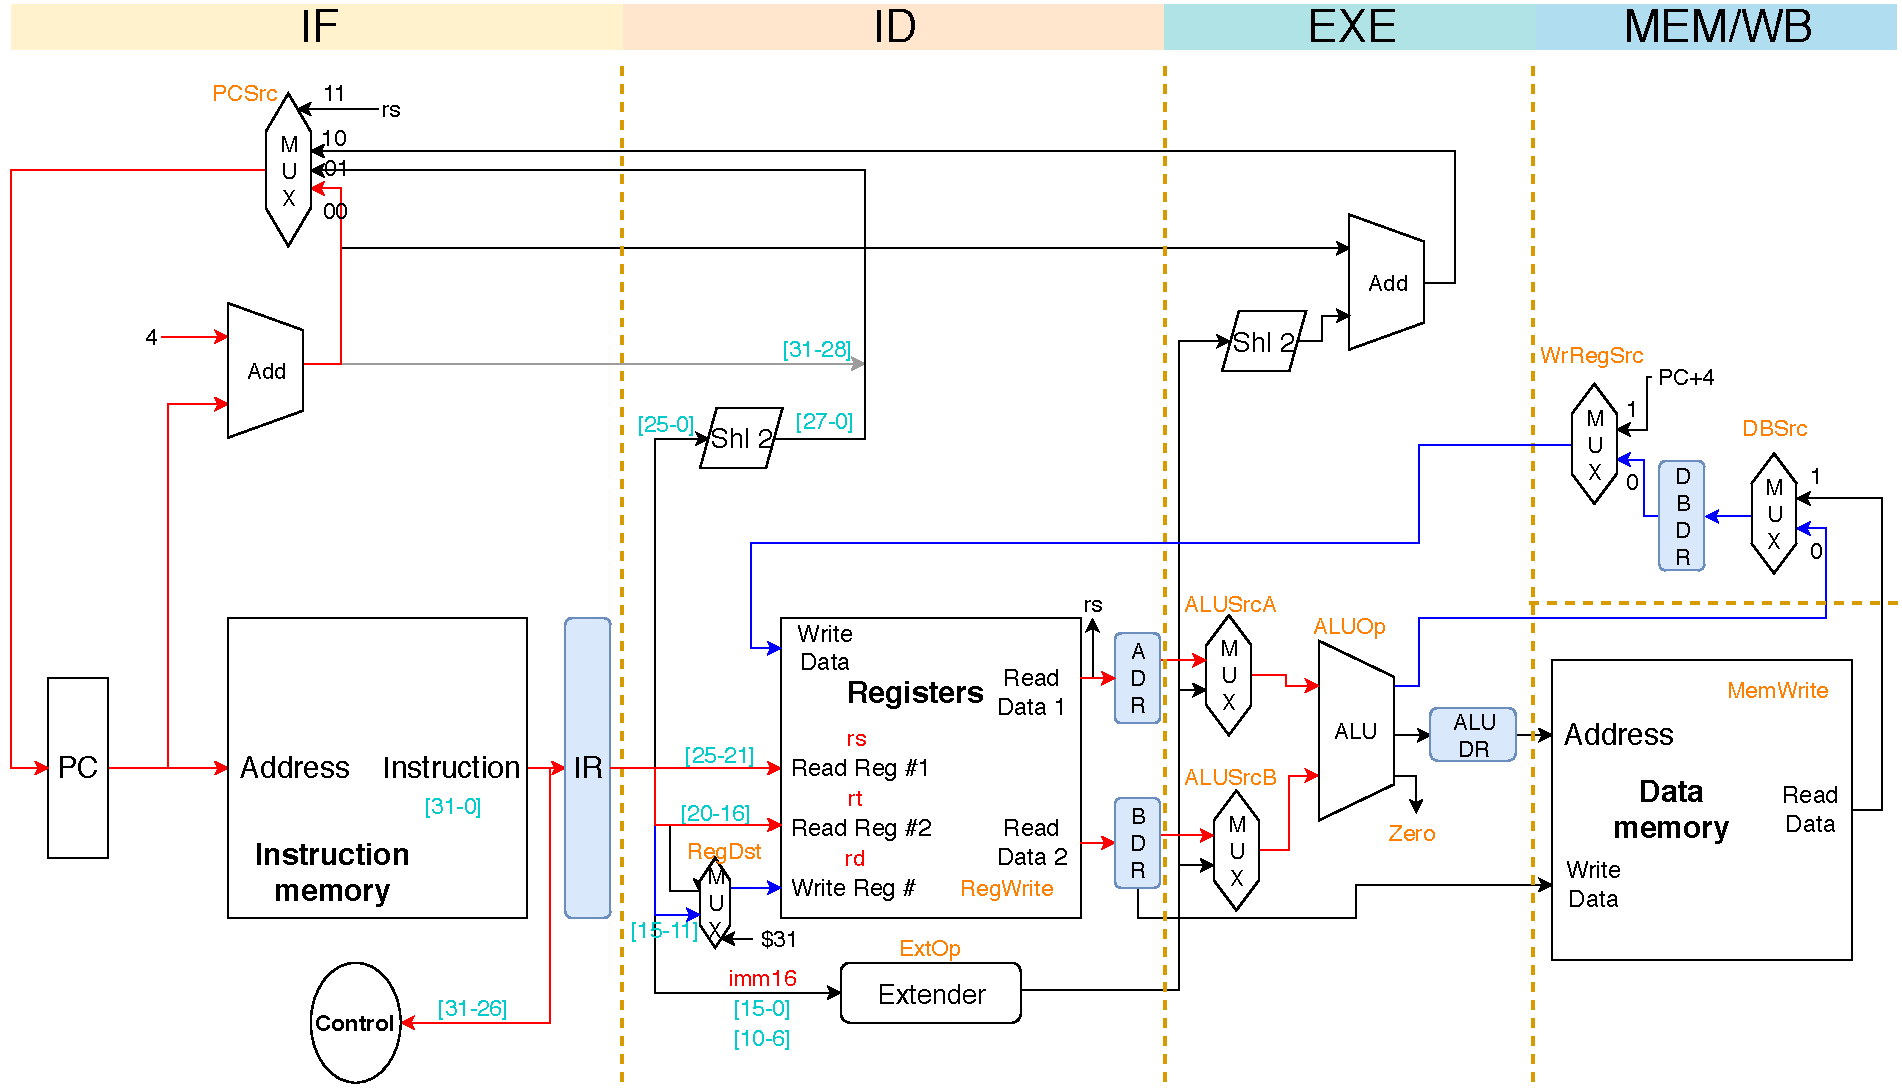
\includegraphics[width=\linewidth]{fig/Datapath-add-sub.pdf}
\caption{Add/sub/and/or/slt通路}
\label{fig:datapath_add}
\end{figure}
\begin{figure}[H]
\centering
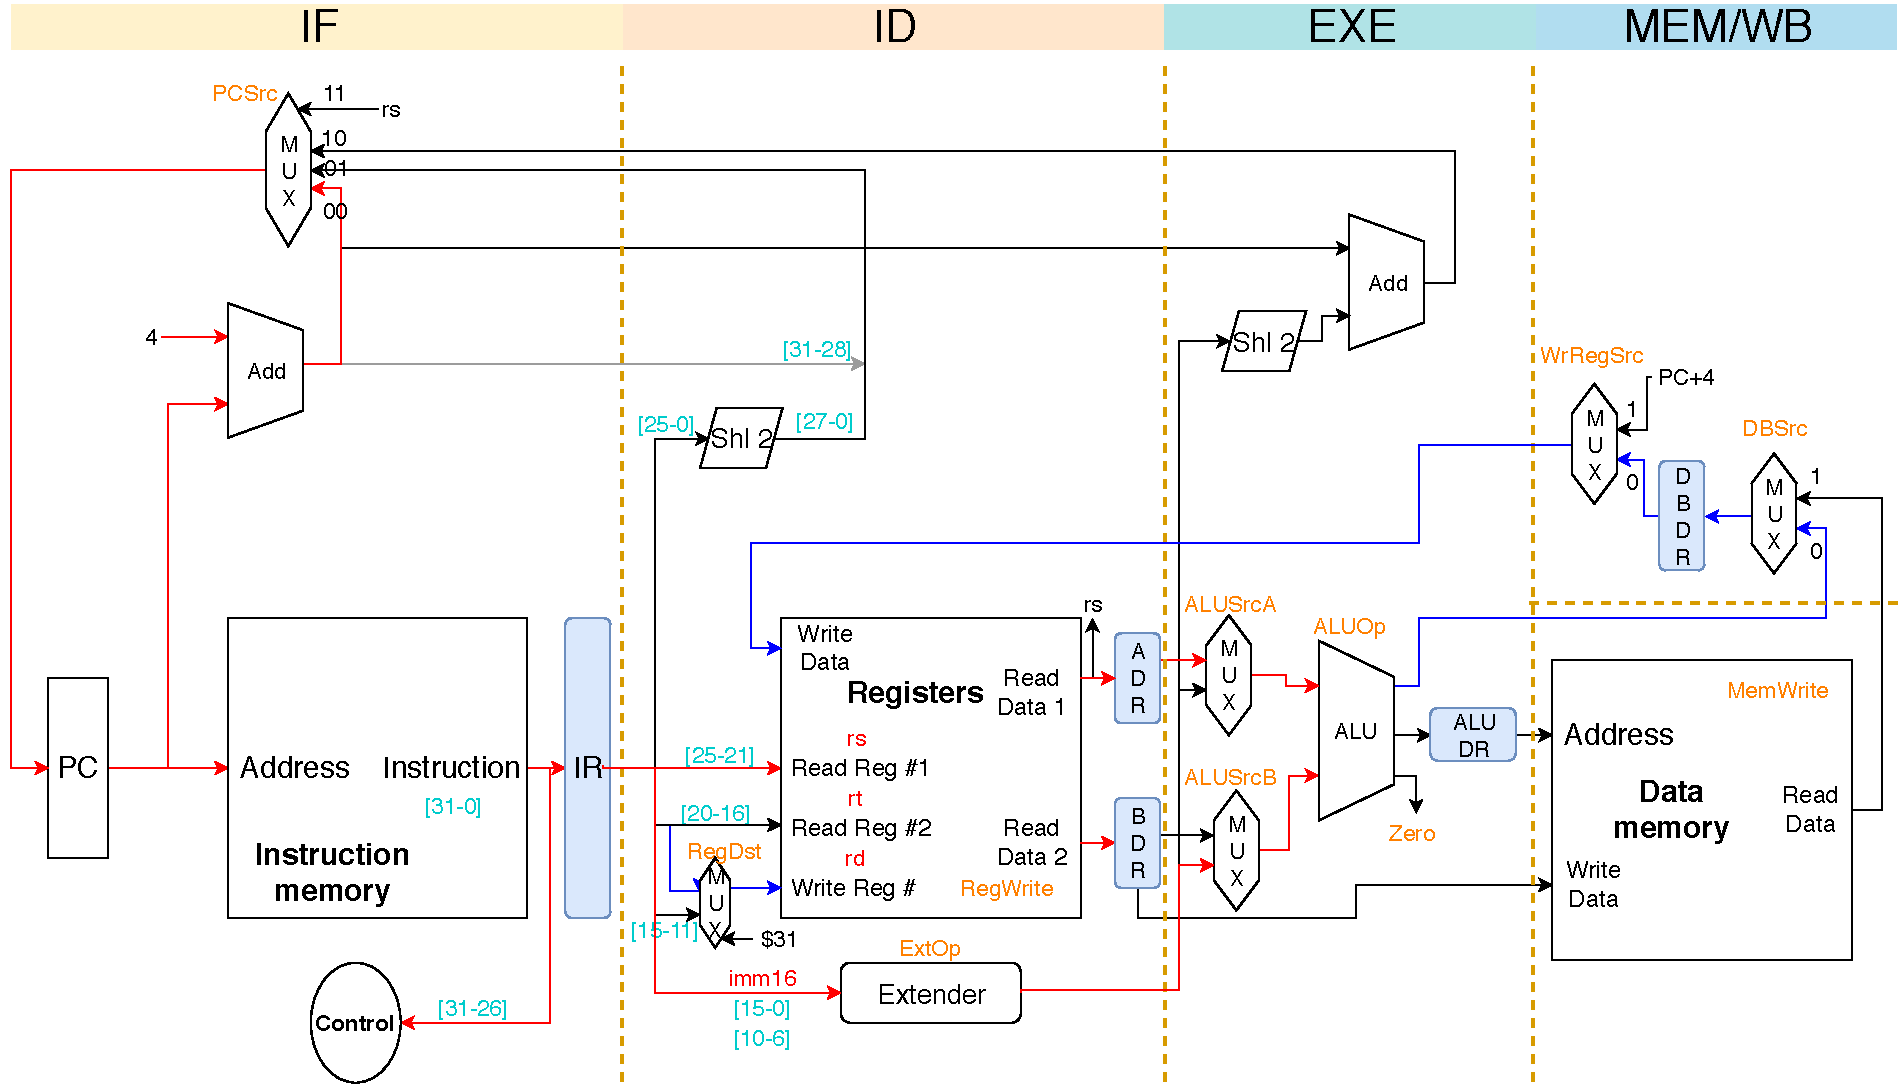
\includegraphics[width=\linewidth]{fig/Datapath-addi-subi.pdf}
\caption{Addiu/andi/ori/xori/slti通路}
\label{fig:datapath_addi}
\end{figure}
\begin{figure}[H]
\centering
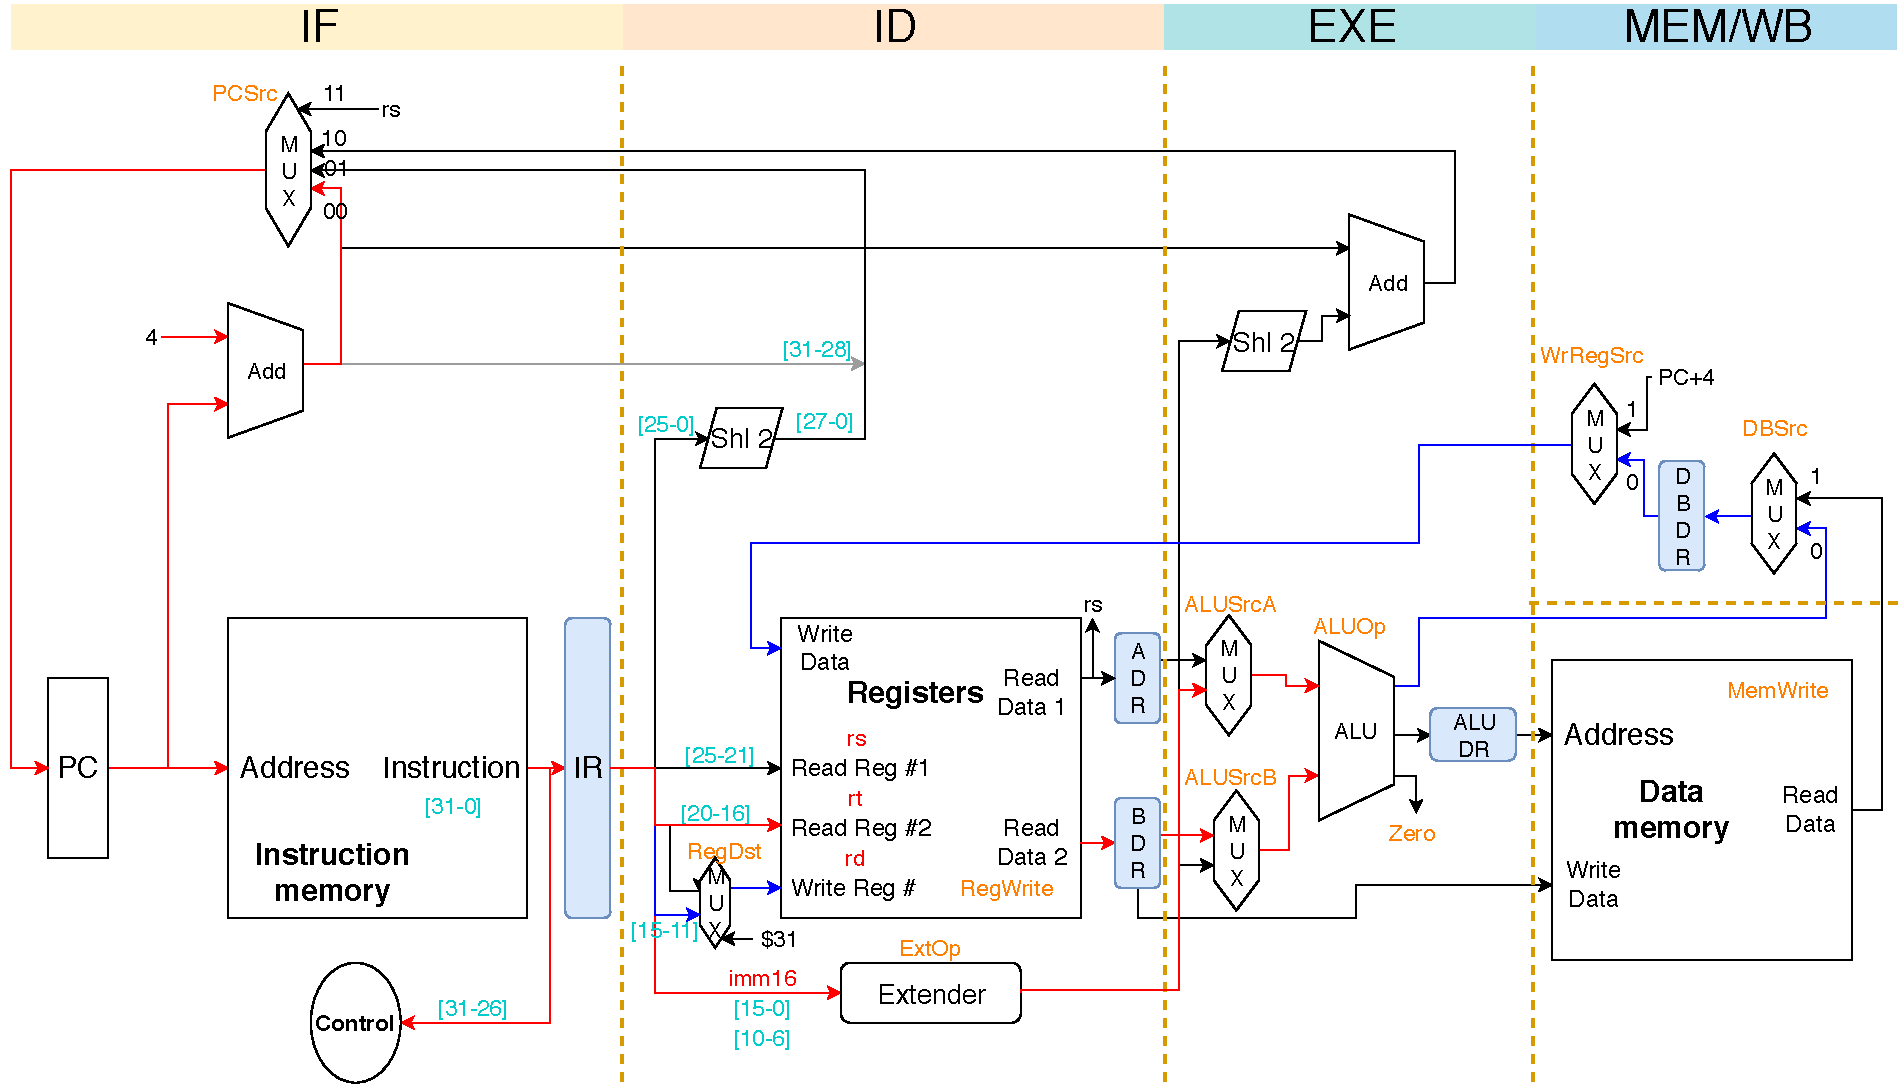
\includegraphics[width=\linewidth]{fig/Datapath-sll.pdf}
\caption{sll通路}
\label{fig:datapath_sll}
\end{figure}

\subsubsection{访存}
\begin{enumerate}
	\item sw为I类型。见图\ref{fig:datapath_sw},执行阶段从指令中读入rs、rt寄存器的地址,对偏移量(imm)进行\textbf{符号}扩展,与rs寄存器的内容相加得到内存地址,将rt寄存器的内容写入内存。
	\item lw为I类型。见图\ref{fig:datapath_lw},执行阶段从指令中读入rs、rt寄存器的地址,rt作为写入寄存器(RegDst=0),对偏移量(imm)进行\textbf{符号}扩展,与rs寄存器的内容相加得到内存地址,将内存的内容写入rt寄存器。
\end{enumerate}
\begin{figure}[H]
\centering
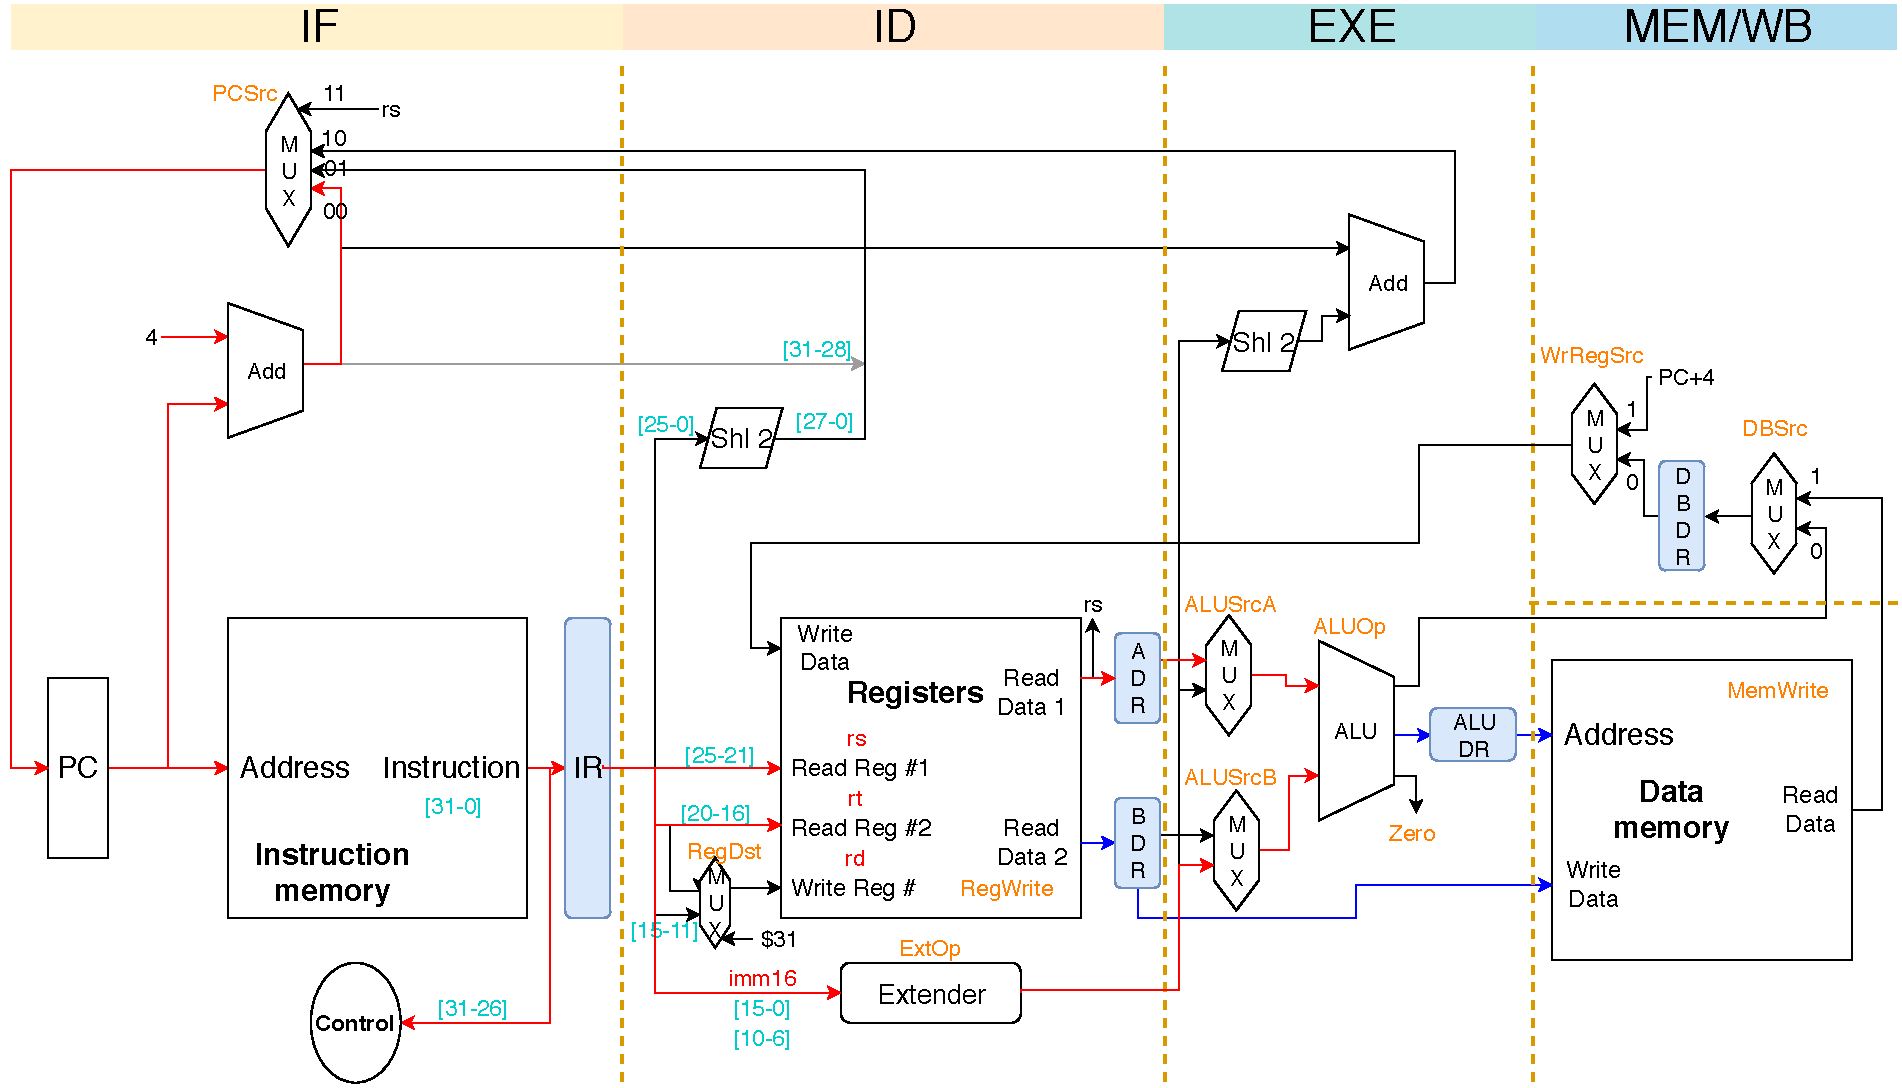
\includegraphics[width=\linewidth]{fig/Datapath-sw.pdf}
\caption{sw通路}
\label{fig:datapath_sw}
\end{figure}
\begin{figure}[H]
\centering
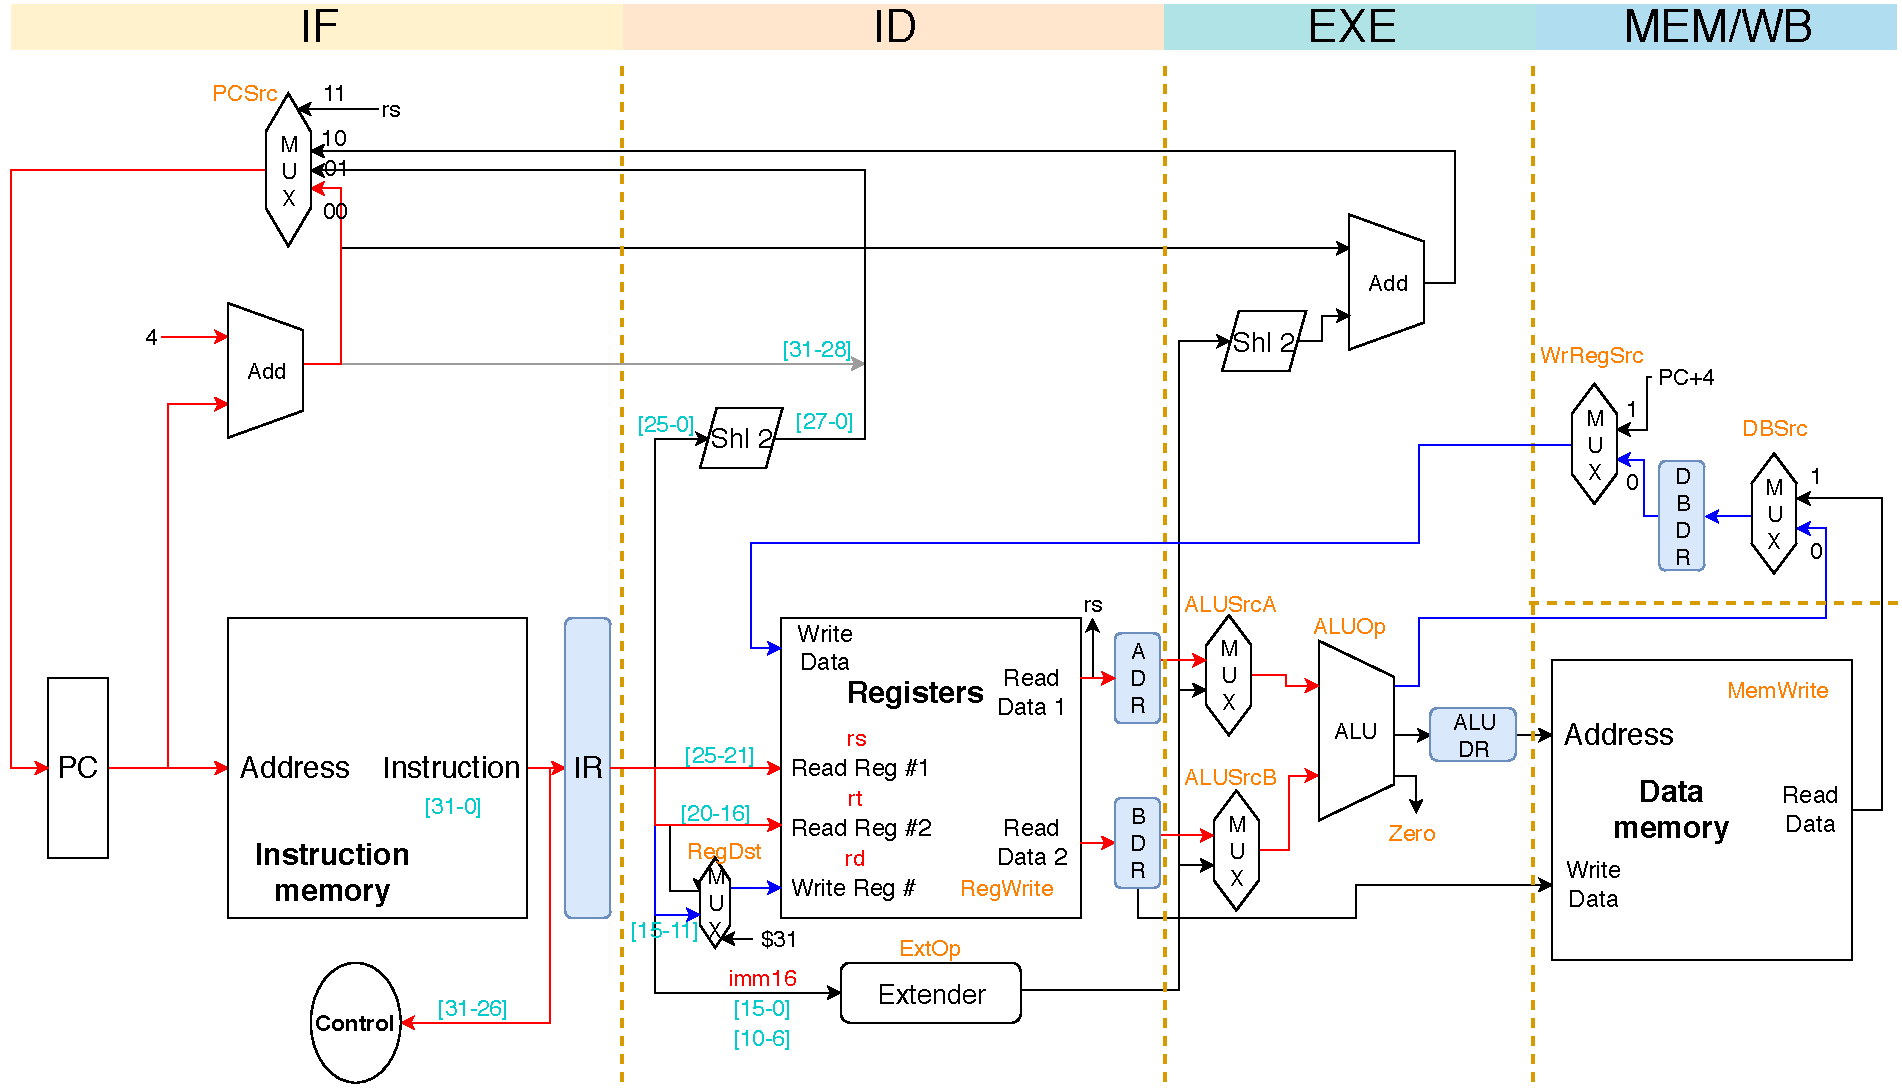
\includegraphics[width=\linewidth]{fig/Datapath-lw.pdf}
\caption{lw通路}
\label{fig:datapath_lw}
\end{figure}

\subsubsection{分支跳转}
\qquad由于MIPS指令为32位(4字节),一般情况下PC每次自增都加4,即PC末两位一定为0,放在指令中(PC偏移/转移地址)即可省略末两位。指令读出时则要左移2位,将末尾的0补齐。
为最大程度利用指令的每一位,跳转指令也是将高4位和低2位都省略掉了,读出时要补回。
\begin{enumerate}
	\item beq/bne/bltz为I类型。见图\ref{fig:datapath_beq},执行阶段从指令中读入rs、rt寄存器的地址,利用ALU对rs、rt寄存器的内容进行相减(beq/bne)或有符号比较(bltz),若结果为0,则Zero标志置1,否则置0;同时,立即数imm进行符号扩展,并左移两位,与原有的PC+4再相加,结合Zero的值得到是否执行分支跳转指令。
	\item j/jal为j类型。j见图\ref{fig:datapath_j},执行阶段直接对指令的低26位左移2位,补上PC+4的高4位,得到跳转地址,更新PC。
	jal的情况类似,见图\ref{fig:datapath_jal},但注意需要将原来的PC+4写入31号寄存器,以便函数调用后返回。
	\item jr为R类型,常用于函数调用后返回,见图\ref{fig:datapath_jr},需要读出rs寄存器的内容,并作为PC的跳转值
\end{enumerate}
\begin{figure}[H]
\centering
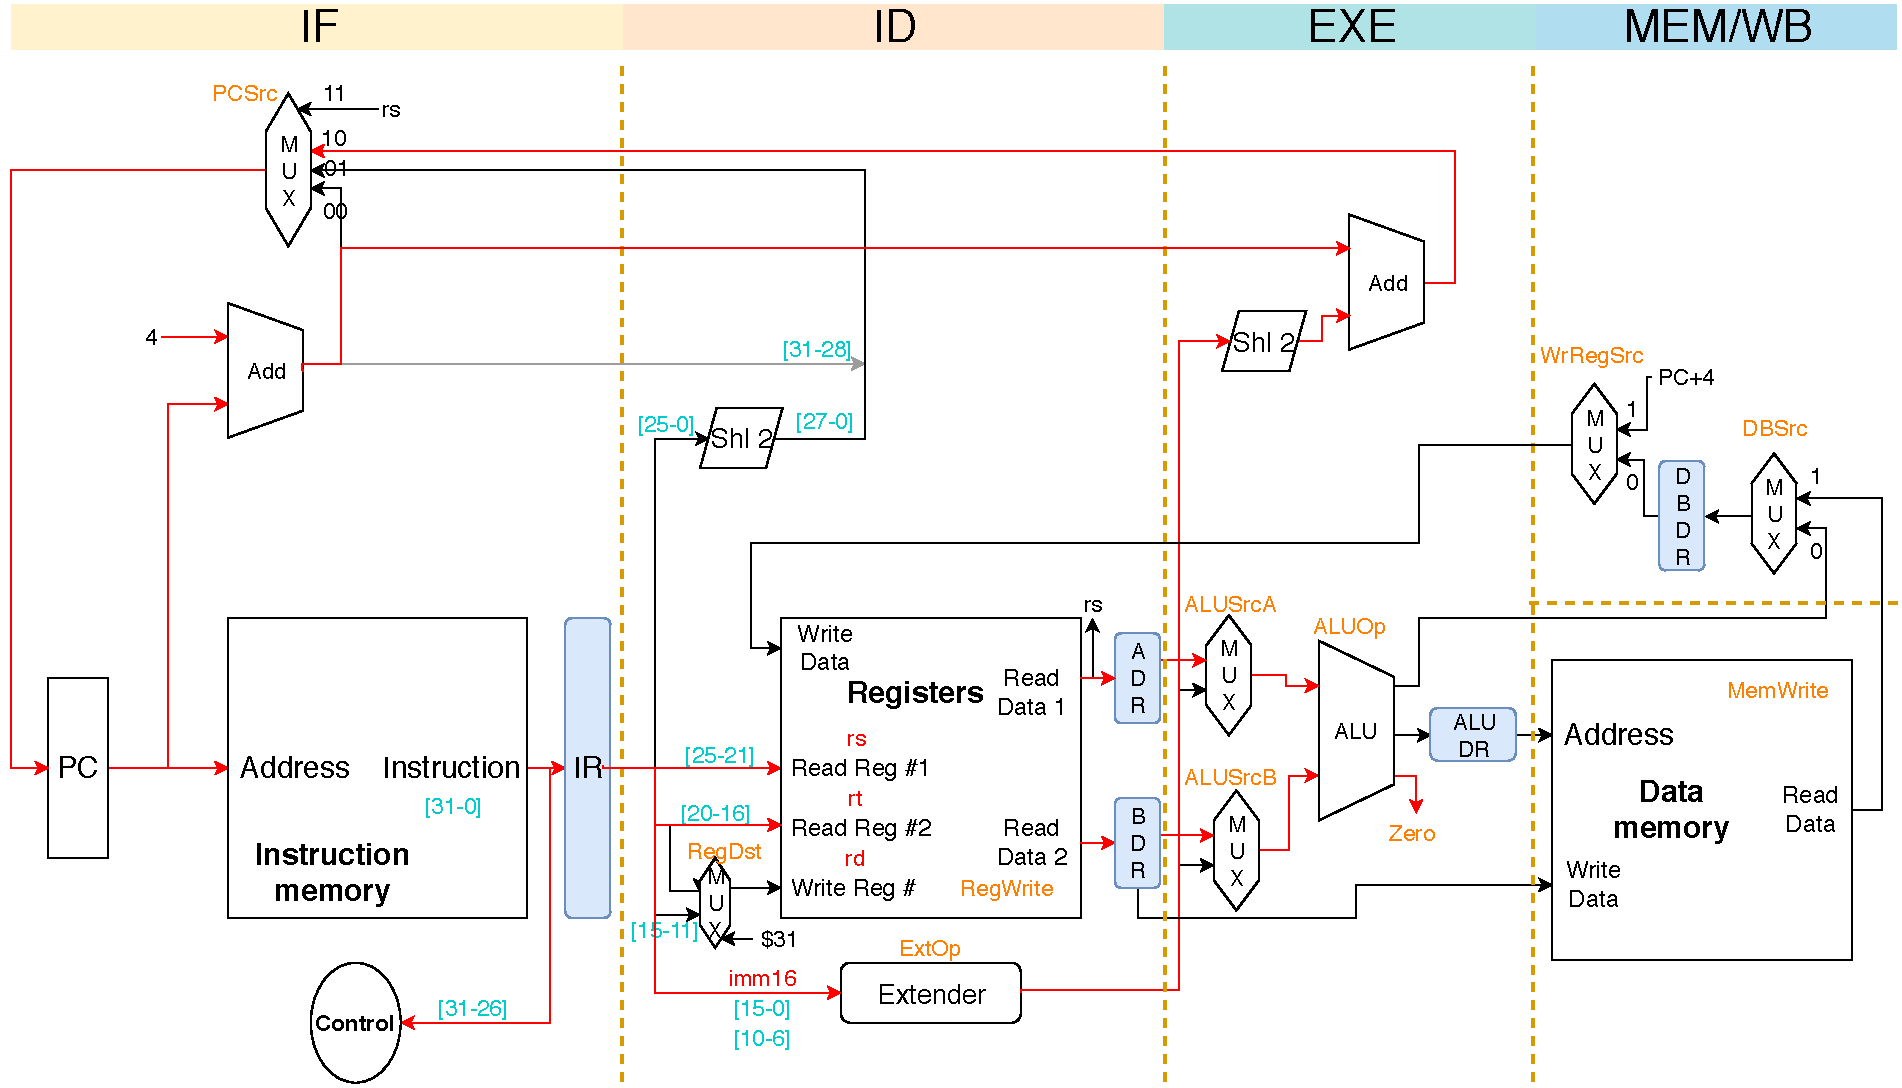
\includegraphics[width=\linewidth]{fig/Datapath-beq.pdf}
\caption{beq/bne/bltz通路}
\label{fig:datapath_beq}
\end{figure}
\begin{figure}[H]
\centering
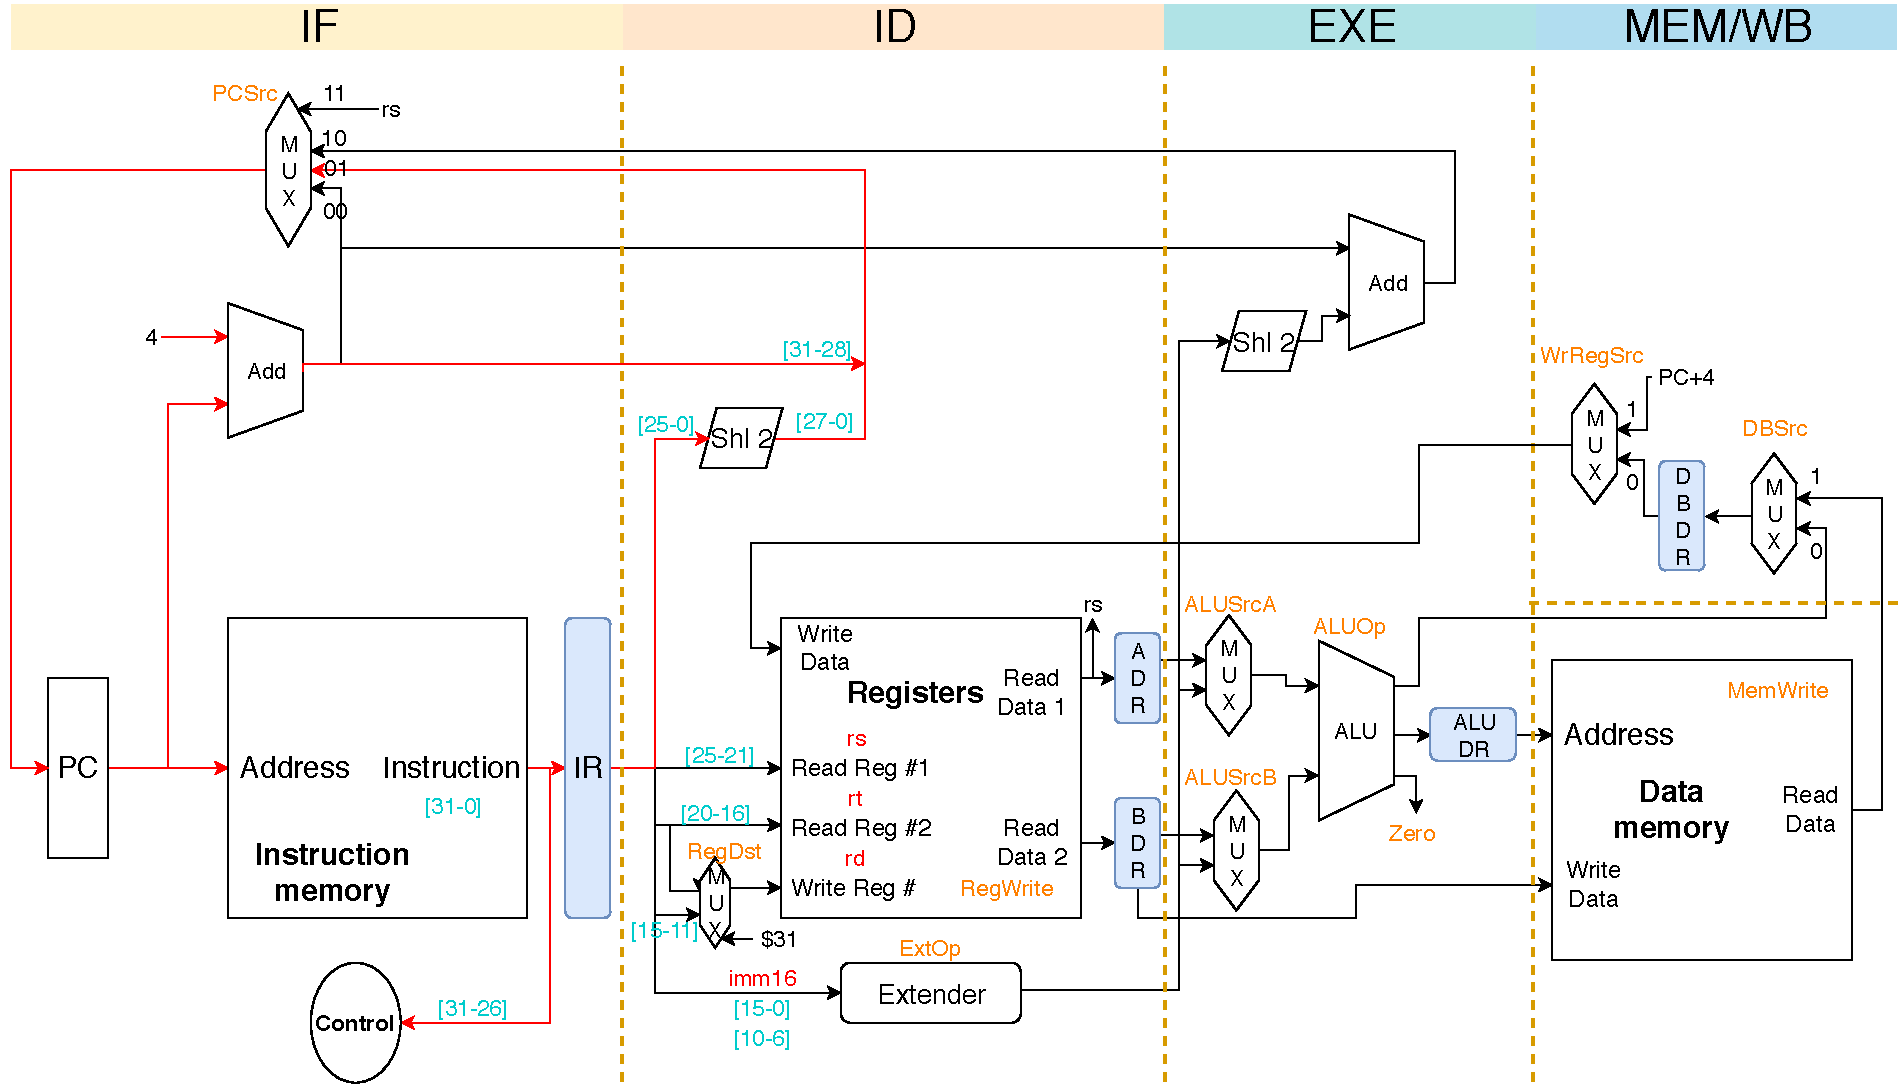
\includegraphics[width=\linewidth]{fig/Datapath-j.pdf}
\caption{j通路}
\label{fig:datapath_j}
\end{figure}
\begin{figure}[H]
\centering
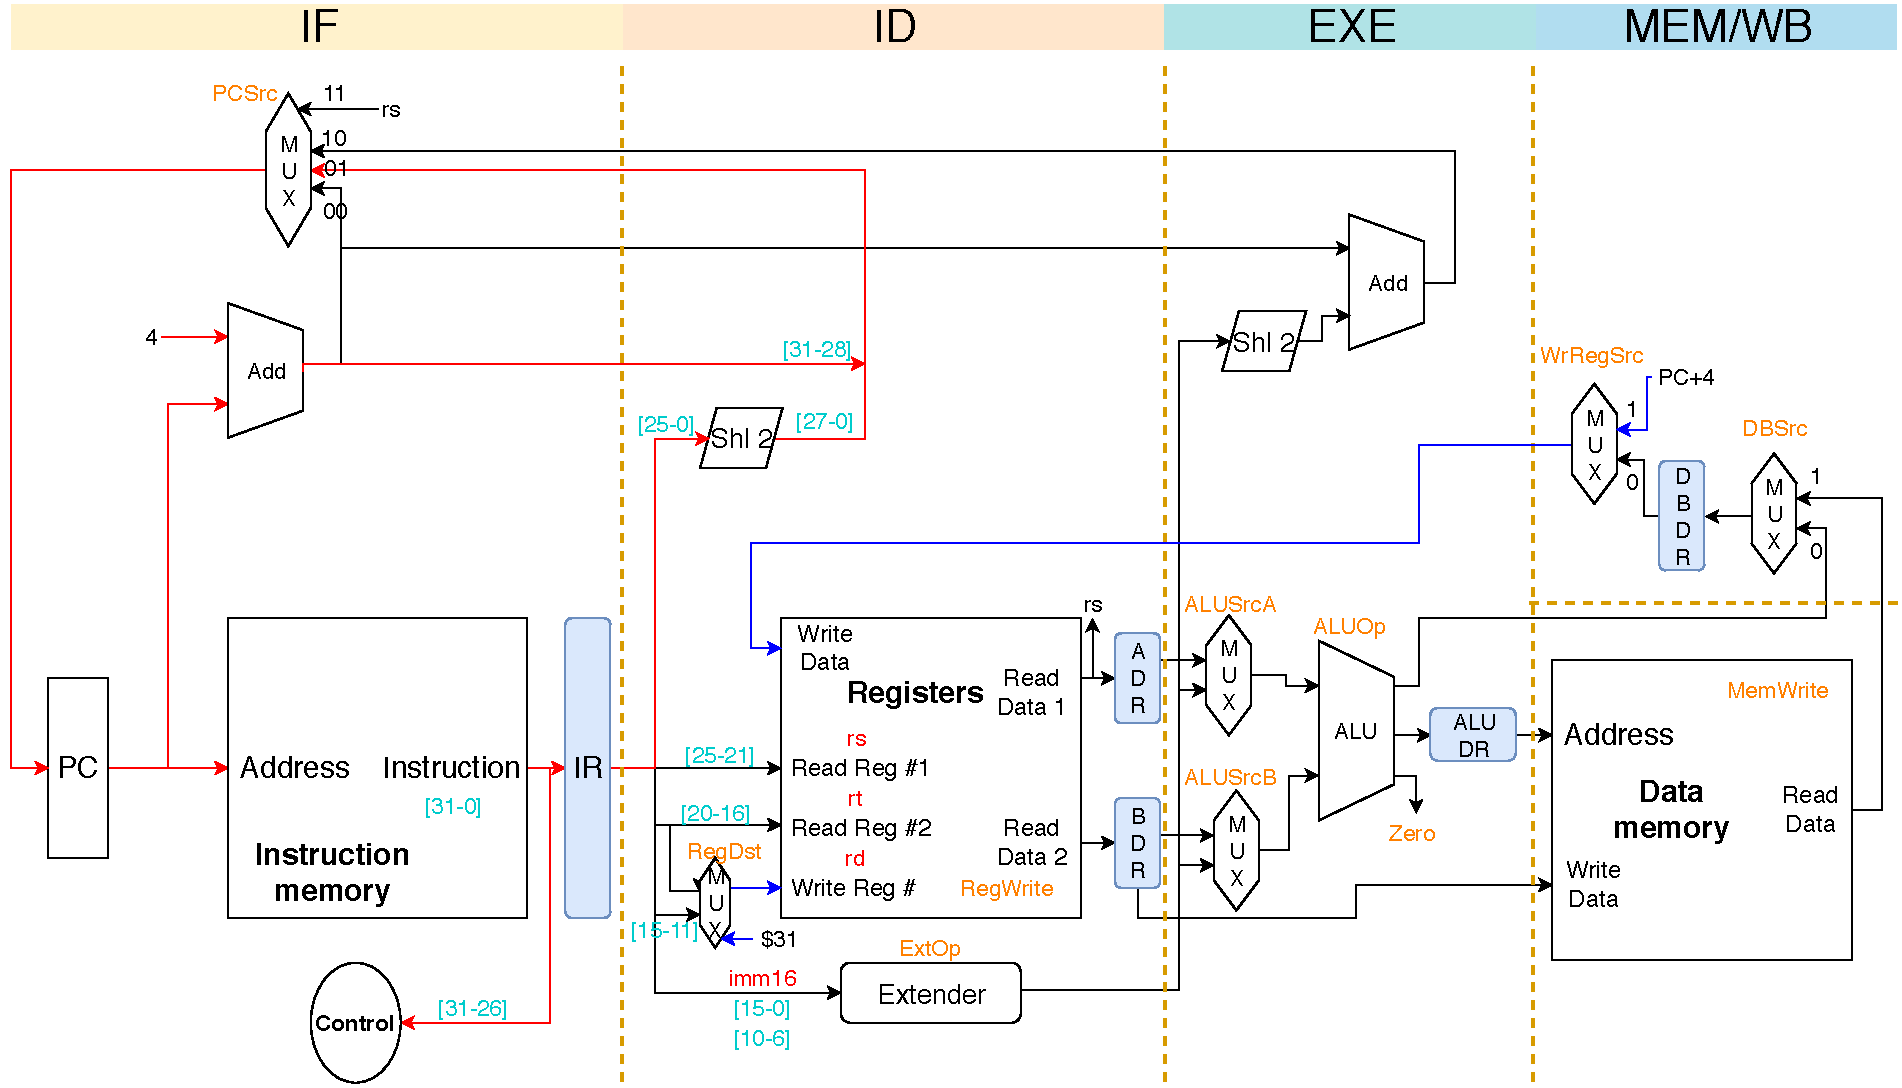
\includegraphics[width=\linewidth]{fig/Datapath-jal.pdf}
\caption{jal通路}
\label{fig:datapath_jal}
\end{figure}
\begin{figure}[H]
\centering
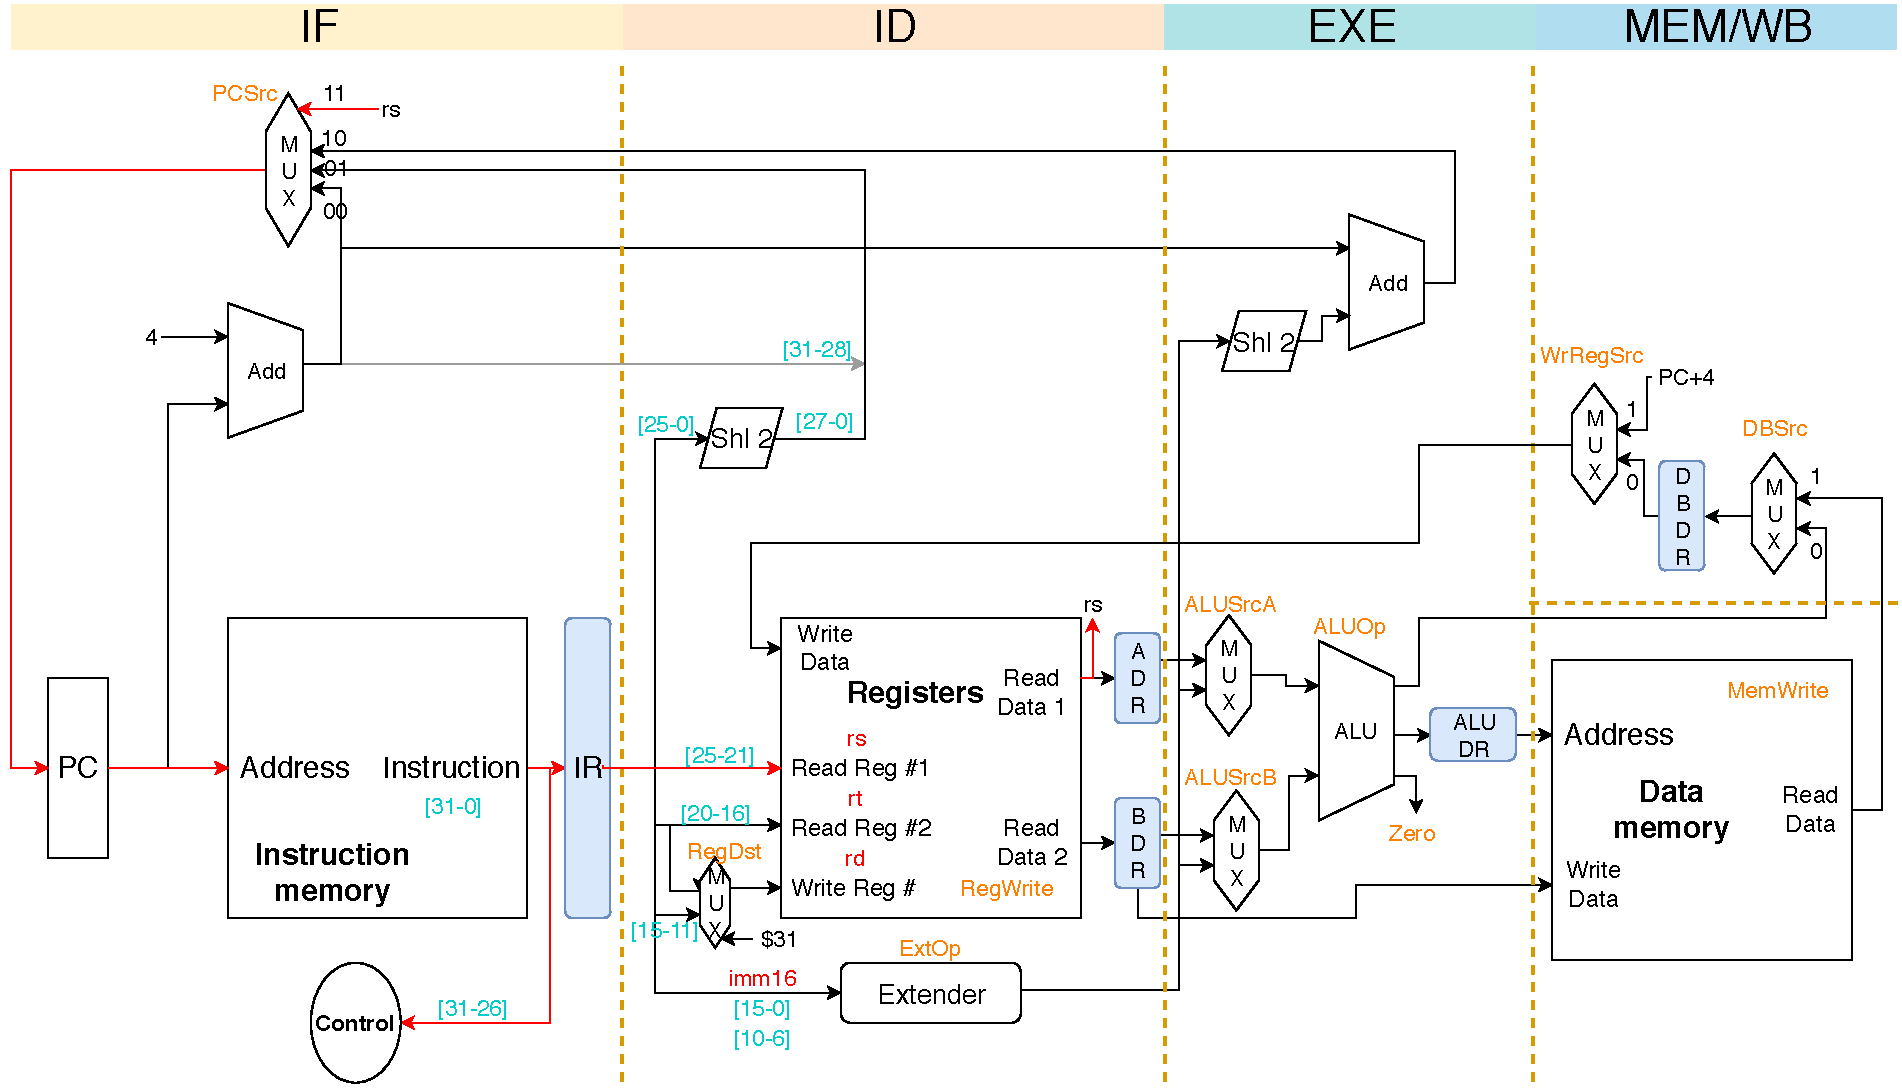
\includegraphics[width=\linewidth]{fig/Datapath-jr.pdf}
\caption{jr通路}
\label{fig:datapath_jr}
\end{figure}

\subsubsection{停机指令}
\qquad PCWrite置为0,不改变PC的值,PC不再变化